% !TEX TS-program = pdfLaTeX+shellescape
% !TEX encoding = UTF-8 Unicode

\documentclass{standalone}
\usepackage{pgfplots}
\pgfplotsset{compat=1.17}
\usepackage{amssymb}

\definecolor{tab_blue}{HTML}{1F77B4}
\definecolor{tab_orange}{HTML}{FF7F0E}

\begin{document}
    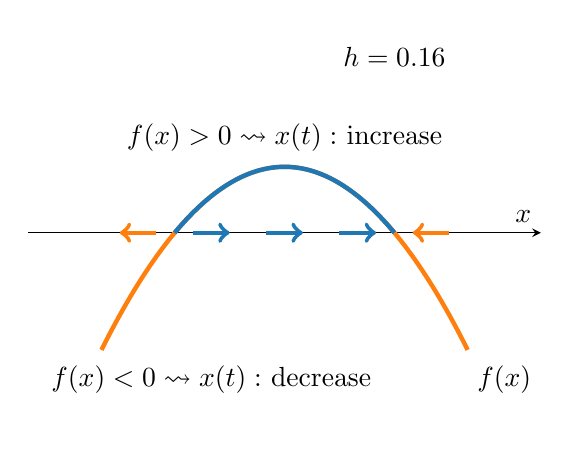
\begin{tikzpicture}[baseline]
        \begin{axis}[
            scale=0.95, % scale
            xmin=-0.2,xmax=1.2,ymin=-0.28,ymax=0.28, % range of plot
            % legend style={at={(axis cs: 1,0)}, anchor=south east}, % position of legends
            unit vector ratio = {1, 2}, % aspect ratio
            axis lines = middle, % middle or box
            %axis x line = bottom, % top, middle, bottom, none: axis x line* = ... removes arrow heads
            %axis y line = left, % left, center, right, none: axis y line* = ... removes arrow heads
            xlabel = {$x$}, % axis labels 
            xtick = {-10},
            y axis line style = {draw=none},
            ytick = {-10},
        ]
            \addplot[color=tab_orange, samples=100, domain=0:1, ultra thick] {-x^2+x-0.16};
            \addplot[color=tab_blue, samples=100, domain=0.2:0.8, ultra thick] {-x^2+x-0.16};
            \node at (0.8, 0.24) {$h=0.16$};
            \node at (0.5, 0.13) {$f(x)>0 \leadsto x(t):$ increase};
            \node at (0.3, -0.20) {$f(x)<0 \leadsto x(t):$ decrease};
            \node at (1.1, -0.20) {$f(x)$};
            \draw[->, color=tab_blue, ultra thick] (0.25,0) -- (0.35,0);
            \draw[->, color=tab_blue, ultra thick] (0.45,0) -- (0.55,0);
            \draw[->, color=tab_blue, ultra thick] (0.65,0) -- (0.75,0);
            \draw[->, color=tab_orange, ultra thick] (0.15,0) -- (0.05,0);
            \draw[->, color=tab_orange, ultra thick] (0.95,0) -- (0.85,0);
            
        \end{axis}
    \end{tikzpicture}
    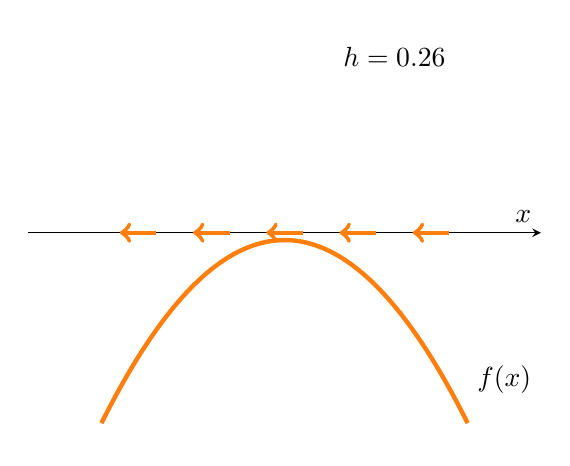
\begin{tikzpicture}[baseline]
        \begin{axis}[
            scale=0.95, % scale
            xmin=-0.2,xmax=1.2,ymin=-0.28,ymax=0.28, % range of plot
            % legend style={at={(axis cs: 1,0)}, anchor=south east}, % position of legends
            unit vector ratio = {1, 2}, % aspect ratio
            axis lines = middle, % middle or box
            %axis x line = bottom, % top, middle, bottom, none: axis x line* = ... removes arrow heads
            %axis y line = left, % left, center, right, none: axis y line* = ... removes arrow heads
            xlabel = {$x$}, % axis labels 
            xtick = {-10},
            y axis line style = {draw=none},
            ytick = {-10},
        ]
            \addplot[color=tab_orange, samples=100, domain=0:1, ultra thick] {-x^2+x-0.26};
            \node at (0.8, 0.24) {$h=0.26$};
            \node at (1.1, -0.20) {$f(x)$};
            \draw[->, color=tab_orange, ultra thick] (0.35,0) -- (0.25,0);
            \draw[->, color=tab_orange, ultra thick] (0.55,0) -- (0.45,0);
            \draw[->, color=tab_orange, ultra thick] (0.75,0) -- (0.65,0);
            \draw[->, color=tab_orange, ultra thick] (0.15,0) -- (0.05,0);
            \draw[->, color=tab_orange, ultra thick] (0.95,0) -- (0.85,0);
        \end{axis}
    \end{tikzpicture}
\end{document}